\documentclass[10pt,letterpaper,onecolumn]{article}
\usepackage{amsmath}
\usepackage{graphicx} 
\usepackage{hyperref}
\usepackage{subfig}
\graphicspath{ {img/} }
\begin{document}
\bibliographystyle{unsrt}
\title{Measuring the Lifetime of a Muon via Double Scintillator Detection\\
\large{Progress Report}}

\author{
 Akhil Deshpande \\*
 Nirmal Patel \\*
 \\*
 PHY 474 Advanced Laboratory \\*
 Spring 2024 \\*
 Dr. Deepa Thomas \\*
 Department of Physics \\*
 The University of Texas at Austin \\*
 Austin, TX 78712, USA
}
\date{\today}
\maketitle
\begin{abstract}
    This experiment utilizes a number of photomultiplier tubes and scintillators to measure the lifetime of muons, elementary particles generated by cosmic rays interacting with Earth's atmosphere. To collect data, we set up a lead glass box, as well as scintillators and photomultiplier tubes to detect when a muon enters the setup. We are currently in the process of determining and analyzing our results.
\end{abstract}
\section{Introduction}
\subsection{Historical Context}
The discovery of the muon in the 20th century marked a pivotal moment in the development of particle physics. Initially observed in cosmic ray experiments by Carl D. Anderson and Seth Neddermeyer at the California Institute of Technology in 1936, \cite{StreetStevenson:1937} the muon ($\mu$) was first mistaken for Yukawa's predicted particle responsible for the nuclear force. Yukawa's meson, theorized in 1935, was expected to mediate the strong interactions within the atomic nucleus, possessing a mass between that of the electron and the proton. However, the properties of the muon, once further analyzed, did not conform to those anticipated for the mediator of the nuclear force. \cite{Yukawa1935}


The muon is a lepton, a class of elementary particles not subject to the strong nuclear force, with a negative electric charge and a mass approximately 207 times that of the electron. \cite{CODATA2018MuonElectronMassRatio} The existence of the muon necessitated a significant expansion of the particle zoo, heralding the beginning of an era that would eventually lead to the establishment of the Standard Model of particle physics.


The clarification of the muon's nature and its differentiation from Yukawa's meson, later identified as the pion ($\pi$), was instrumental in the advancement of quantum field theories. This distinction emphasized the need for a comprehensive framework to understand the plethora of particles being discovered. The subsequent development of quantum electrodynamics (QED) and the electroweak theory, which unified the electromagnetic and weak forces, were partially motivated by the necessity to incorporate the muon and other leptons in a coherent theoretical structure. \cite{MuonG2Experiment2004}
\subsection{Theoretical Background}

The muon ($\mu$) is an elementary particle in the lepton family, akin to the electron but with a significantly greater mass. It carries a charge of $-1e$ and has a spin of $\frac{1}{2}$, classifying it as a fermion under the Standard Model of particle physics. The muon's mass is approximately $105.7 \, \text{MeV}/c^2$, making it about 207 times more massive than the electron. Despite its greater mass, the muon decays to an electron, a neutrino, and an antineutrino, due to the weak interaction, showcasing its unstable nature.

\subsubsection{Muon Decay}

The primary decay mode of the muon is represented by the following equation:
\[
\mu^- \rightarrow e^- + \bar{\nu}_e + \nu_\mu
\]
This decay process is mediated by the weak force, specifically through the exchange of a $W^-$ boson in the virtual state. The Feynman diagram for this decay illustrates the muon decaying into a muon neutrino and a virtual $W^-$ boson, which then converts into an electron and an electron antineutrino. The half-life of the muon in its rest frame is approximately $2.2 \, \mu\text{s}$, a duration that, while brief, allows for extensive experimental study of its decay processes and the verification of the Standard Model predictions. \cite{Beringer2012Leptons}

\subsubsection{Cherenkov Radiation}

When a muon travels through a medium at a speed greater than the phase velocity of light in that medium, it emits Cherenkov radiation, a phenomenon analogous to a sonic boom but with electromagnetic waves. The radiation is emitted at a characteristic angle $\theta$ relative to the direction of the particle's motion, which can be described by the formula:
\[
\cos\theta = \frac{1}{n\beta}
\]
where $n$ is the refractive index of the medium and $\beta$ is the speed of the particle relative to the speed of light in vacuum. 
\cite{Jackson1999Electrodynamics}

\section{Experimental Procedure}
\subsection{Apparatus}
\subsubsection{Overview}
This experiment focuses on detecting the presence of muons through the use of scinillators and photmultiplier tubes. We first set up a plastic scintillator on top of a lead glass box. This top scintillator will detect when a muon first passes through it. Then, the lead glass box will capture the muon, slowing it to rest. The muon will then decay, as shown above. The decay components will be measured by either a left of a right photomultiplier tube (PMT). When these PMTs activate, these signals are timed by our ORTEC setup, and we can achieve a spectrum of the lifetimes of the captured particles. 

An alternate setup we can consider is in the case of a single PMT and scintillator setup. We can wire this setup to a time-to-amplitude (TAC)converter directly. When the muon enters the scintillator, it will activate the PMT, and when it decays, it will again activate the PMT. This difference in times is measured by the TAC, and sorted into 'bins' by a multi-channel analyzer (MCA), such that it again provides us with an exponential decay spectrum.
\begin{figure}
    \begin{center}
        \subfloat[\centering MCA, TAC, and time calibrator]{{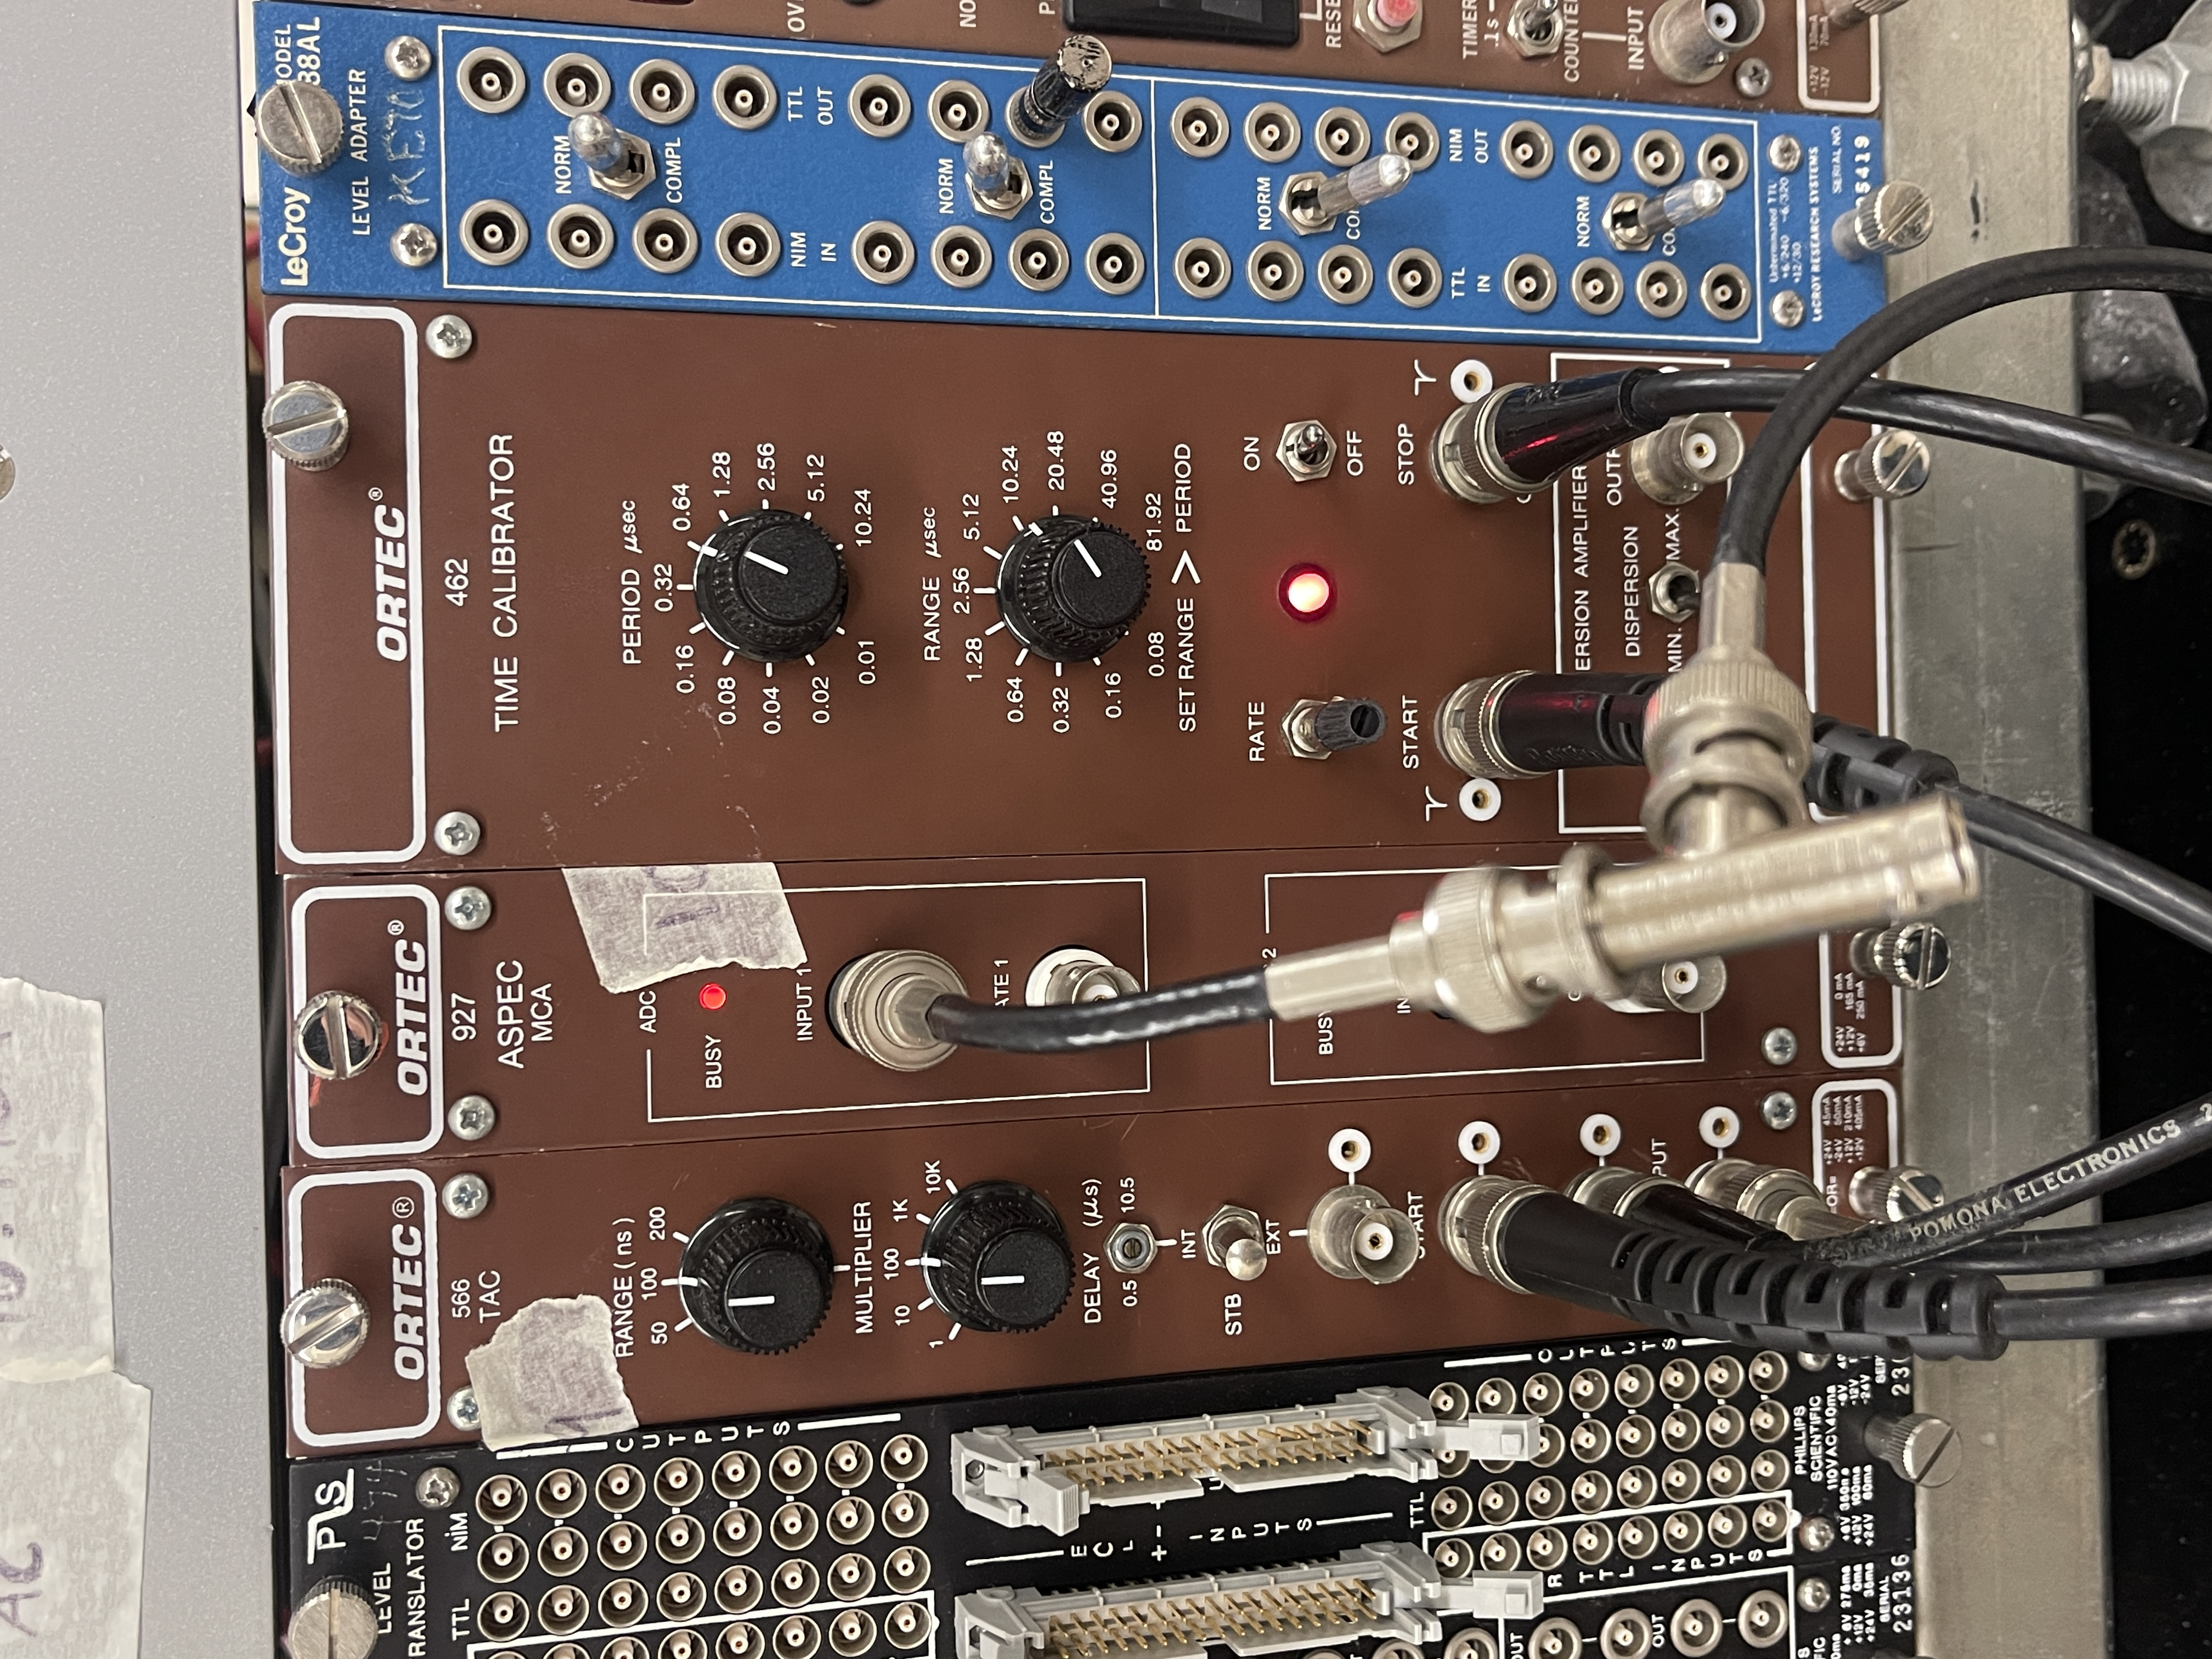
\includegraphics[width=6cm, angle = 270]{Apparatus009.JPG}}}%
        \qquad
        \subfloat[\centering Philips Components]{{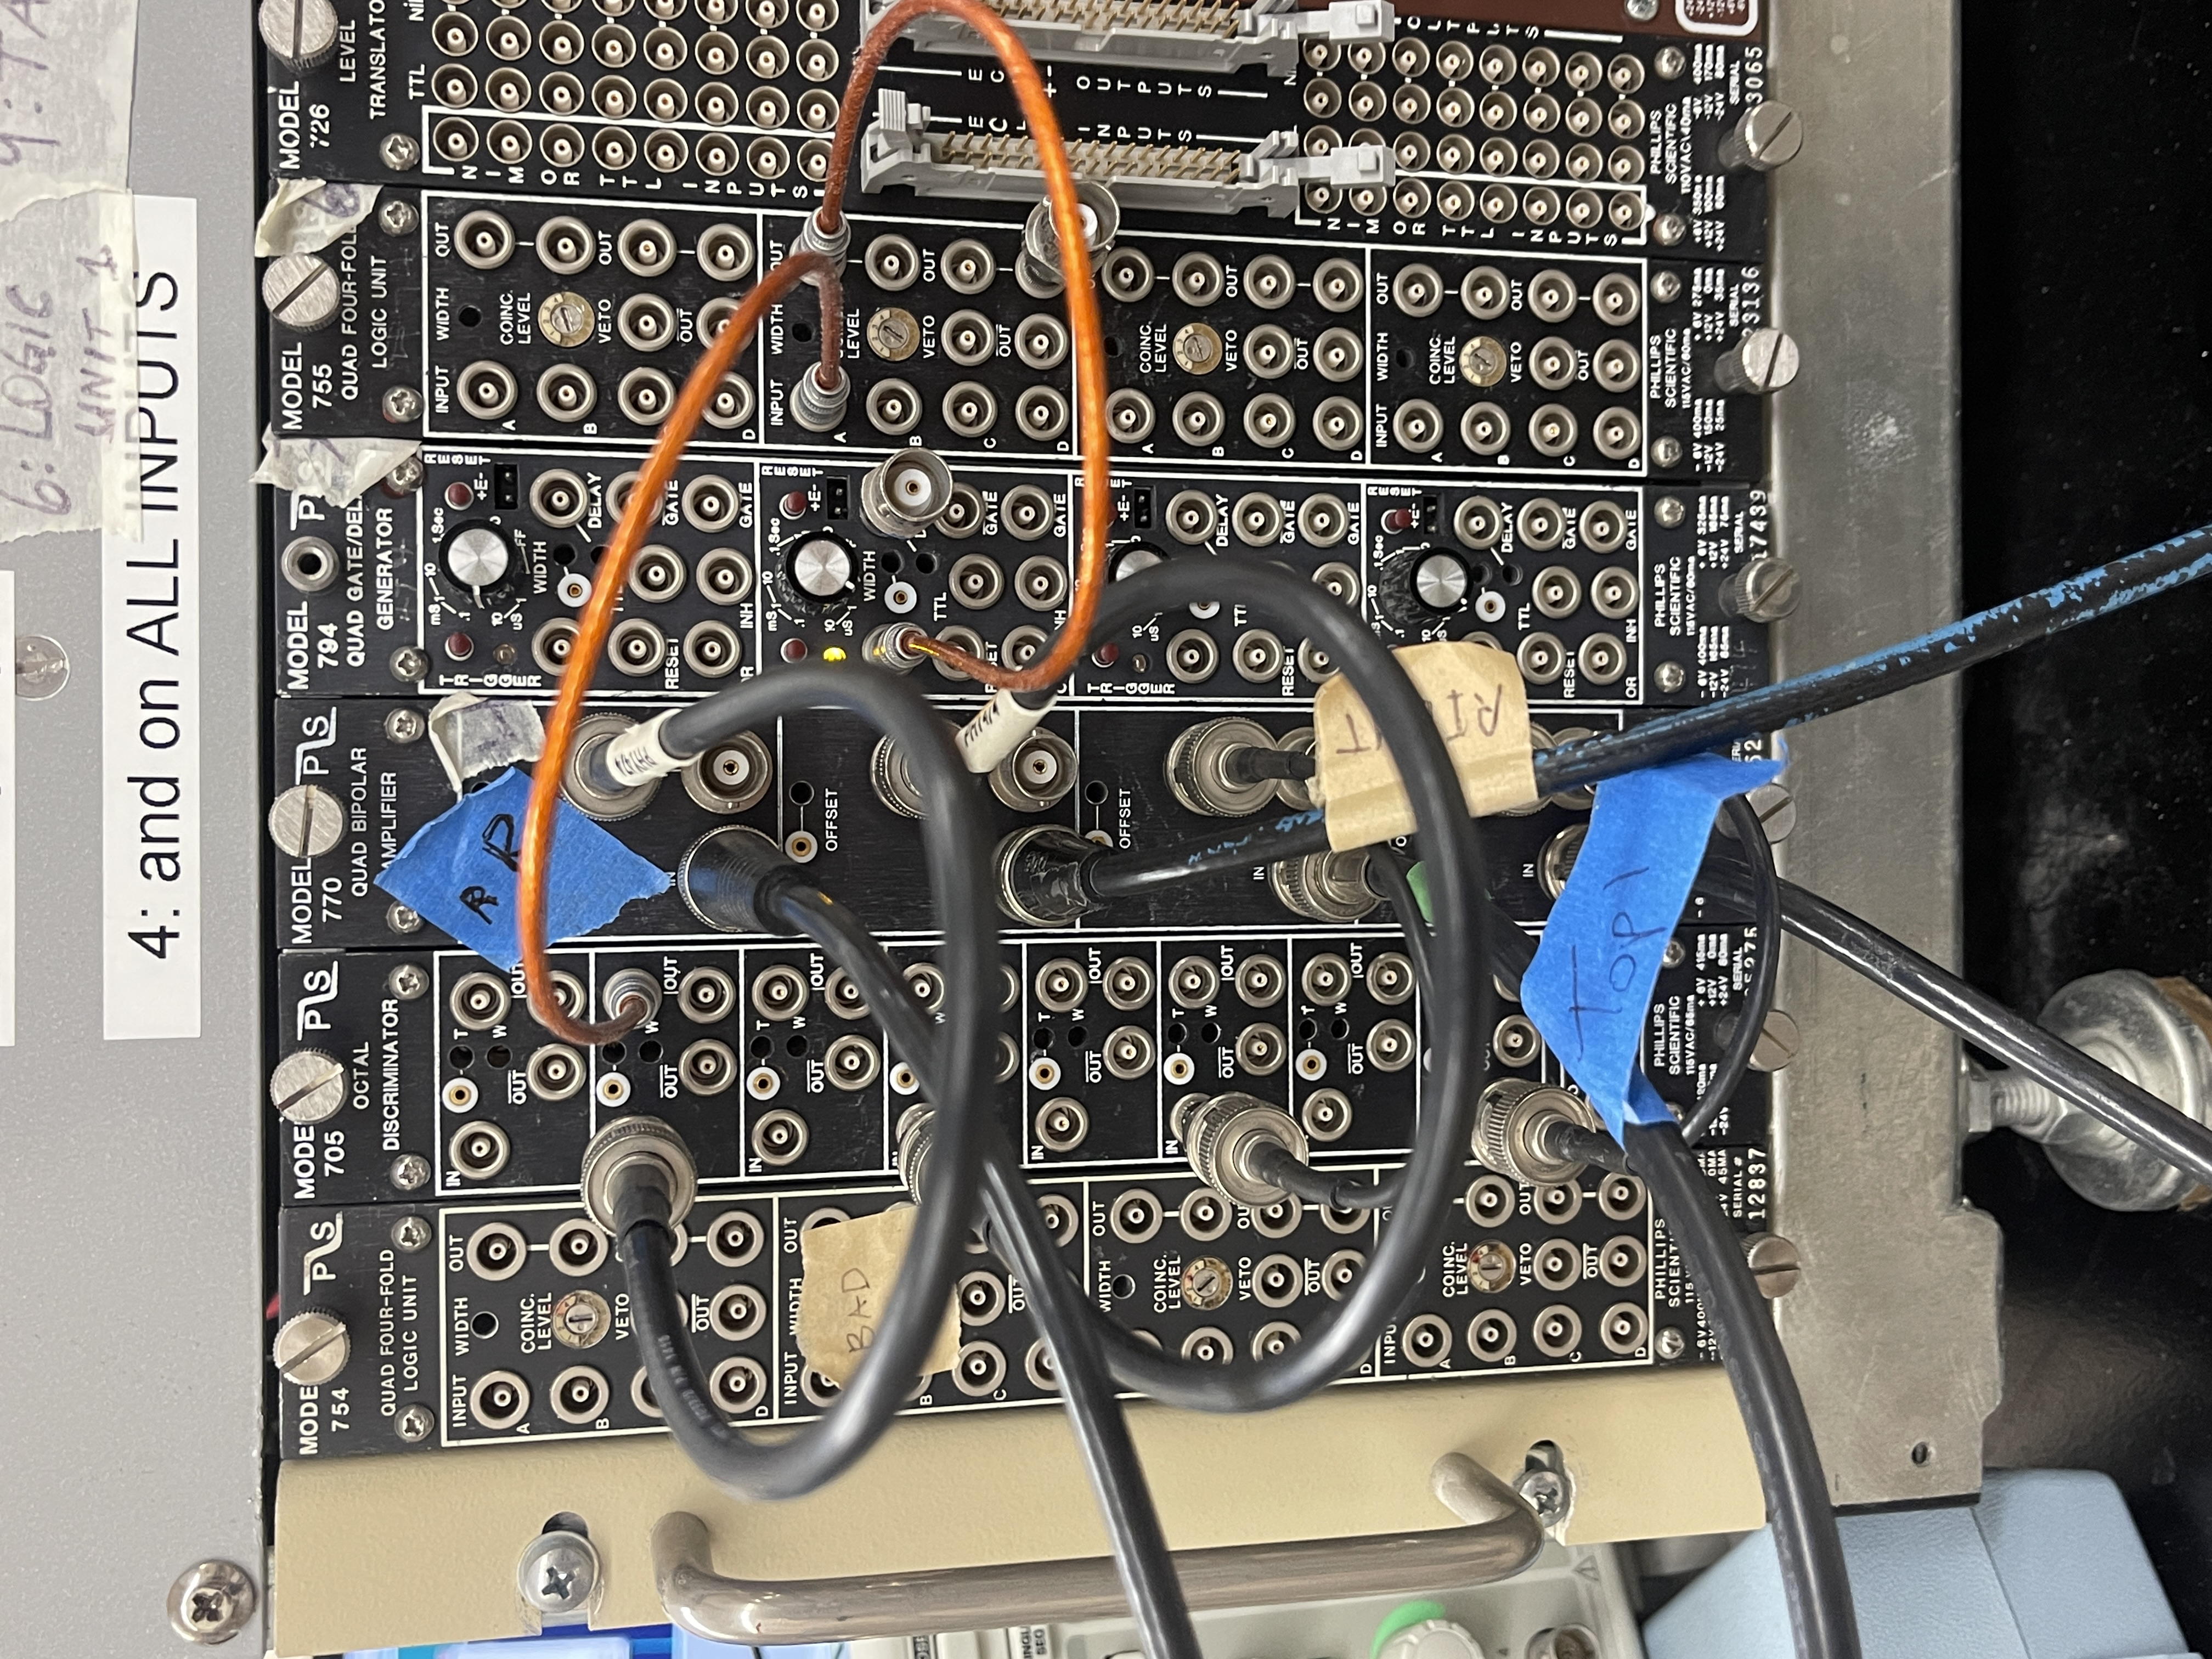
\includegraphics[width=6cm, angle = 270]{Apparatus008.JPG} }}%
        \caption{Here, we have the Philips components, shown on the right. These include the logic component, delay generator and discriminator. On the left, we have our MCA, TAC, and time calibrator, which were manufactured by ORTEC.}%
        \label{fig:apparatus}%
    \end{center}
\end{figure}
\subsubsection{Photomultiplier Tube}

A Photomultiplier Tube (PMT) is a highly sensitive photodetector that is widely utilized in the detection and measurement of low levels of light, ultraviolet (UV), and near-infrared (NIR) radiation. The device operates on the principle of photoelectric effect combined with secondary emission to achieve a high level of signal amplification. A typical PMT consists of a photoemissive material coated cathode, a series of dynodes, and an anode.


The operational mechanism of a PMT begins with the absorption of incident photons by the photoemissive cathode, leading to the emission of photoelectrons due to the photoelectric effect. These photoelectrons are then accelerated towards the first dynode by an electric potential difference. Upon colliding with the dynode, each photoelectron induces the emission of multiple secondary electrons. This process is repeated across a series of dynodes, each at a progressively higher potential, resulting in an exponential increase in the number of electrons. The amplified electron stream finally reaches the anode, producing a measurable current that is proportional to the intensity of the incident light. 

A photo of one our photomultiplier tubes can be found in Figure \ref{fig:rightpmt}. This is the rightmost PMT in our setup.

\begin{figure}[hbt!]
    \begin{center}
        {{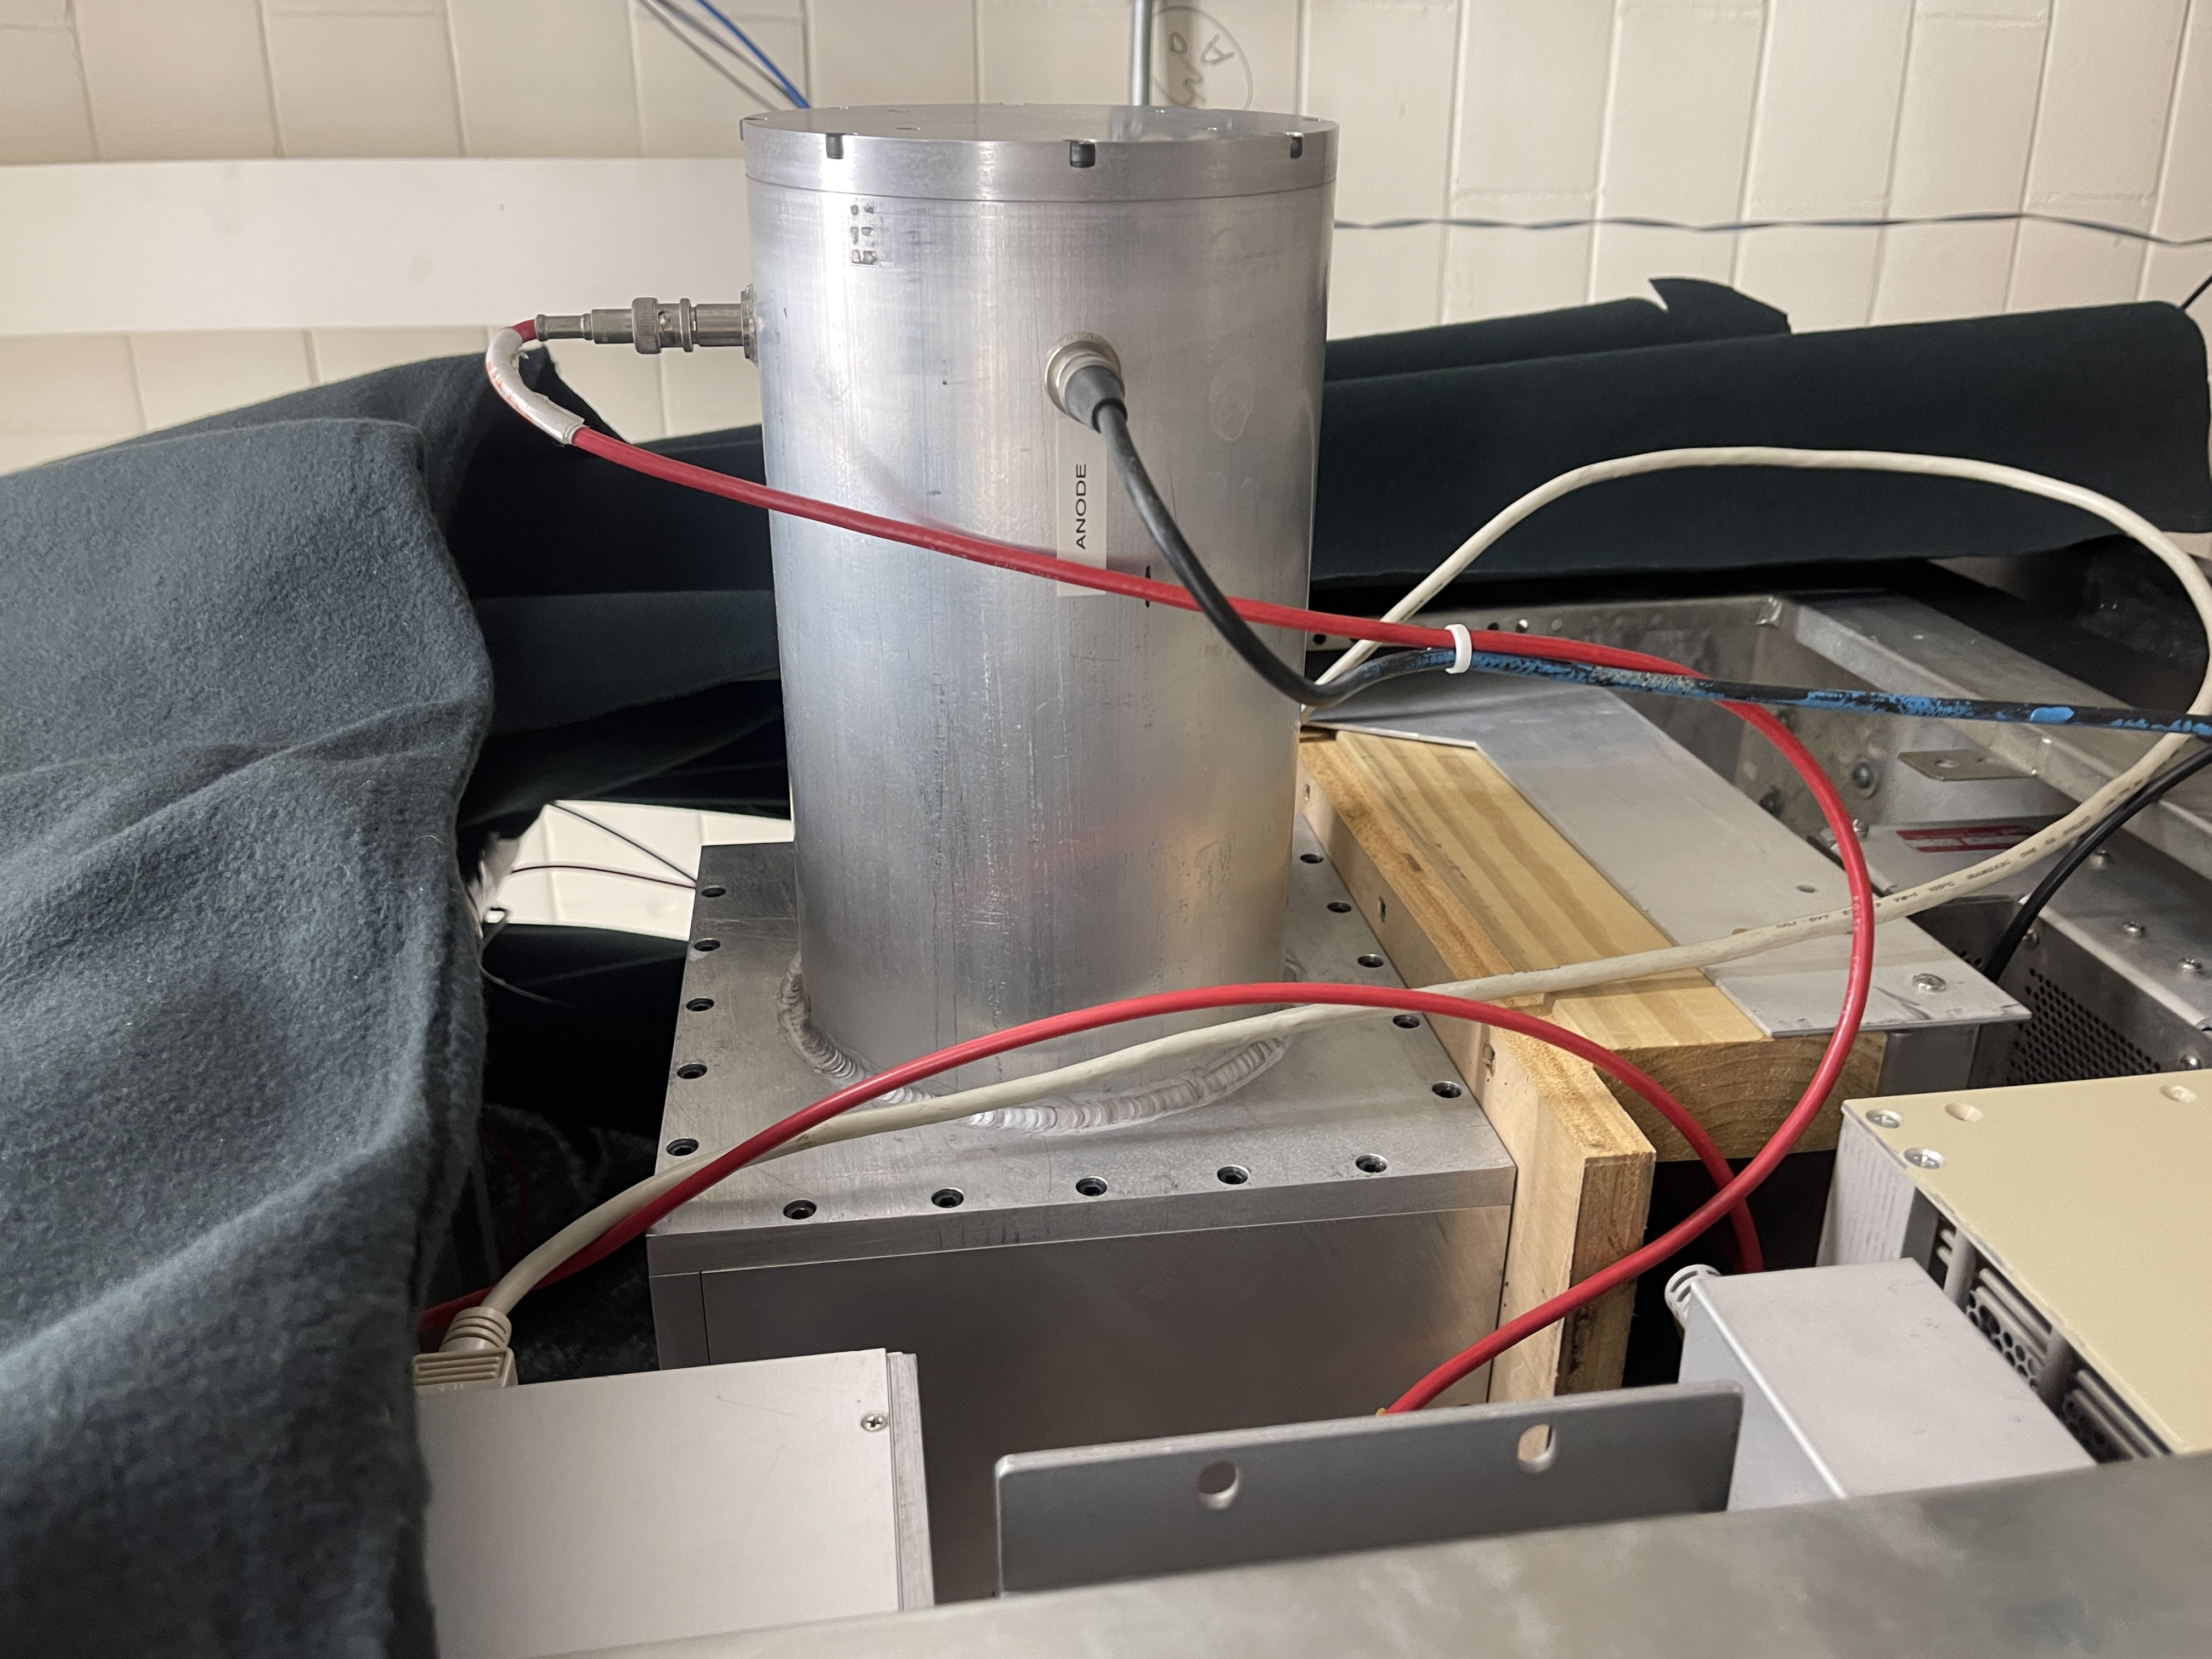
\includegraphics[width=7cm, angle = 270]{Apparatus001.JPG} }}%
        \caption{A picture of our rightmost photomultiplier tube. This tube, and its left counterpart were used to take data, as they are directly attached to the lead glass box.}%
        \label{fig:rightpmt}%
    \end{center}
\end{figure}
\subsubsection{ORTEC and Philips Components}
The main ORTEC and Philips Components are the ORTEC 462, 927, and 566, as well as the Philips 705, and 755, as well as a high voltage power supply.

The Philips 705 and 755 are the discriminator unit and the logic unit, respectively. The discriminator allows for the exclusion of false signals from any input, and the logic unit allows us to perform logical operations (such as AND and OR) on our signals.

The ORTEC 462 is a time calibrator, used to calibrate our time measurements. The ORTEC 566 is a time-to-amplitude converter (TAC). This is used to differentiate the time between a start and a stop signal. The output of this TAC is piped into the ORTEC 927, which is our multi-channel analyzer (MCA). THe MCA counts are then output to our computer. A loose photo can be seen in Figure \ref{fig:apparatus}
\subsubsection{Computer Software}
To capture the output from the MCA, we use MAESTRO, a software that plots the MCA's counts in a human-readable format. 
\subsection{Data Collection}
We are currently in the process of collecting data. This involves letting our setup run for long periods of time, and observing the spectrum of counts we achieve from our MCA. As of 3/28/24, we are conducting a four-day long trial to determine if our latest wiring setup is accurate.
\begin{figure}[hbt!]
    \begin{center}
        {{\includegraphics[width=8cm]{Apparatus000.JPG} }}%
        \caption{A photo of our high-voltage power supply. Each knob and dial combination directs a voltage to the corresponding PMT or scintillator it is wired to. We set our voltage to 1.1 kV.}%
        \label{fig:psu}%
    \end{center}
\end{figure}
\section{Data Analysis}
We are currently in the process of analyzing our data
\subsection{Calibration}
We are currently in the process of retrieving more calibration data, as we recently identified a major flaw in our earlier method. However, calibration involves setting an ORTEC 462 Time Calibrator to a variety of different times, then running these signals through our TAC. From there, we run our TAC output to our MCA, and we can identify how the MCA's 'bins' correlate to real world times.
\subsection{Error and Uncertainty}
Right now, much of our anticipated error stems from muons escaping the box, or passing through the box at odd angles. Currently, we are thinking of ways to mitigate this error, but we are leaning toward the process of only using one PMT and scintillator, as this somewhat eliminates the need for the other, more tedious (and error concerning) setup options.
\section{Results and Conclusions}
\subsection{Results}
We currently have no relevant results.
\subsection{Conclusion}
In conclusion, we are extremely close to completing the setup portion of this experiment. The goal of this experiment is to observe muons and determine their lifetime, and so far, we have been able to observe these particles in a lab setting, but are unable to produce or show any concrete data to support this deduction.
\paragraph*{Acknowledgments}
I would like to thank my lab partner, Nirmal Patel for his assistance on data collection. Furthermore, I'd like to thank Dr. Deepa Thomas, Matthew Dwyer, and Erick Martinez for their assistance throughout the measurement and set up processes. 

\section{Next Steps}
\subsection{Wiring and Setup}
As our current wiring and setup are proving unsuccessful, we have several new wiring ideas retrieved from previous lab reports. Furthermore, we have our own ideas that differ due to our bottom scintillator being out of commision.
\newpage
\bibliography{refs} 

\end{document}

